\section{Plik US-PAN-8-10x-echo.dcm}
\begin{frame}
  \frametitle{Plik US-PAN-8-10x-echo.dcm}

  \begin{figure}
    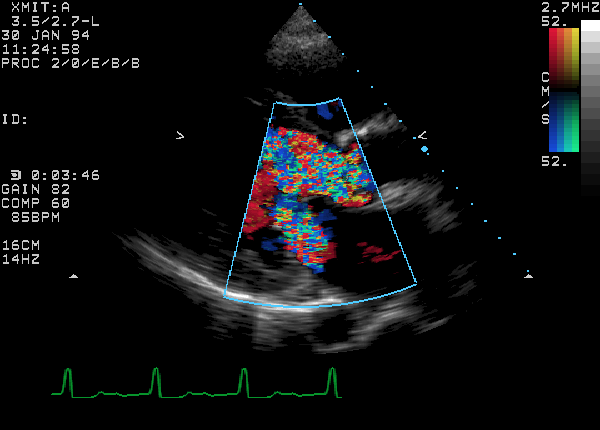
\includegraphics[width=0.4\textwidth]{echo}
  \end{figure}
\end{frame}

\begin{frame}
  \frametitle{Informacje ogólne}
  \begin{itemize}
    \item Kodowanie: Explicit
    \item Długość pliku: 483610B, (481194B danych obrazowych, 99\% pliku)
    \item Plik używa grupowania elementów danych
  \end{itemize}
\end{frame}

\begin{frame}
  \frametitle{Dane identyfikujące - \texttt{0x0008}}

  \begin{itemize}
    \item Badanie: Echokardiogram
    \item Data badania (30 styczna 1994 roku, 11:25)
    \item Sprzęt (ACME Products)
  \end{itemize}
\end{frame}


\begin{frame}
  \frametitle{Informacje o pacjencie - \texttt{0x0010}}
  \begin{center}
    Pacjent w tym pliku jest z anonimizowany.
  \end{center}
\end{frame}

% Sposób pozyskania danych obrazowych - 0018 - nic ciekawego
% Zalezności - 0020 - mało interesujące rzeczy

\begin{frame}
  \frametitle{Informacje o obrazie - \texttt{0x0028}}
\begin{itemize}
  \item Obraz indeksowany
  \item Ilość obrazów: 10
  \item Rozmiar 430x600
  \item Format piksela: 8 bitowa liczba całkowita bez znaków
  \item Format wyjściowy tablicy przekodowań kolorów: 16 bitowe RGB
  \item Zapisane palety kolorów
\end{itemize}
\end{frame}
